\documentclass[a4paper,12pt,oneside]{book}
\usepackage{stata}
\usepackage{graphicx}
\usepackage{tikz}
\usepackage{multirow}
\usepackage{rotating}
\usepackage{tabularx,booktabs}
\newcolumntype{Y}{>{\centering\arraybackslash}X}
\setlength{\parskip}{1em}
\setlength{\parindent}{0pt}
\renewcommand{\baselinestretch}{1.5}
\begin{document}
\begin{titlepage}
    \begin{center}
        \vspace*{1cm}
 
        \Huge
        \textbf{An Introduction to Factor Analysis}
 
        \vspace{0.5cm}
        \LARGE
        Theory and Application
 
        \vspace{1.5cm}
 
        \textbf{Najib A. Mozahem}
 
        \vfill
 
        \vspace{0.8cm}
 
    \end{center}
\end{titlepage}
\tableofcontents
\chapter{Factor Analysis - The Theory}
\section{Introduction}
In statistics, we are interested in recording the values of certain variables. For example, if we wanted to study the academic performance of 
students, then we would record the GPA values. If we wanted to measure the performance of the defence of a certain sports team then we would
record the number of goals that the team has conceded. In these instances, the variable that we are measure is easily quantified. However, what if
we wanted to measure something that was more abstract? For example, what if we wanted to measure an invdividual's time management skills? How can
we do this? What is the number that represents someone's time management skills? 

In cases such as these, we need to resort to measuring the variable of interest using a set of questions. For example, we might ask the individual
to rate himself or herself on the following:

"I am not easily distracted when I am working on something important."

"I do not find it difficult to work on projects that require a lot of effort even if the due date is close."

"I would rather work on important work now even if I do not find it enjoyable instead of do something that I enjoy."

"I find it easy to plan my week ahead of schedule"

We would expect that an individual who has good time management skills would tend to agree with the above four statements while an individual
with weak time management skills would tend to disagree with the statements. In this case, we are measuring time management skills using more than one
question, or more than one variable. The respondents might be asked to answer on a scale of one to five (strongly disagree, disagree, neutral, agree,
strongly disagree) or even on a scale of one to seven. 

This is where factor analysis is used. It is used to measure variables that cannot be captured by a single question or number. In this case, the 
variable of interest, which is time management skills in this case, is made up of, or constructed from, several other variables. This is why such
variables are referred to as constructs. Factor analysis allows us to calculate a single value from the responses of the above questions for each
individual. This way we can quantify the construct "time management skills". 

\section{Example: Masculinity}
As an example, consider that we might want to measure how masculine someone is. Usually, traits that are associated with men include competitivness, 
risk taking behavior, and individualism. Therefore, in order to measure the consctruct "Masculinity", we might ask the respondents to rate
themselves on the traits found in Table ~\ref{table:masculine1}. We would expect that masculine individuals would state that the traits apply to them
while individuals who are not masculine would state that the traits to do not apply to them.  

\begin{table}
\caption{Masculine traits \label{table:masculine1}}
\begin{tabularx}{\textwidth}{ c| *{7}{Y} }
	\hline
	{Trait} & \multicolumn{7}{|c}{(1) Not at all, (7) Applies to me a lot} \\
	\hline
	assertive & 1 & 2 & 3 & 4 & 5 & 6 & 7 \\
	competitive & 1 & 2 & 3 & 4 & 5 & 6 & 7 \\
	dominant & 1 & 2 & 3 & 4 & 5 & 6 & 7 \\
	makes decisions easily & 1 & 2 & 3 & 4 & 5 & 6 & 7 \\
	individualistic & 1 & 2 & 3 & 4 & 5 & 6 & 7 \\
	\hline
\end{tabularx}
\end{table}

\section{Reliability}
After we gather the responses of the individuals we would need to calculate the value of the construct "Masculinity". However, before we do this, it
is very important that we test what is called the reliability of the instrument. Here the word instrument refers to the instrument, or tool, that we
used to measure the construct, which is simply the five questions shown in Table ~\ref{table:masculine1}. 

What do we mean by reliability? Simply that the questions being asked are actually measuring the same construct. We claimed that rating to what
extent the five traits apply to you are a way of measuring the single construct Masculinity, but is this claim plausible? If the five traits do
actually measure the same construct, then we would expect that individuals in general would respondent in a smilar fashion to all of the questions.
For example, if the instrument used is reliable, then an individual who beleives thet he or she is assertive would also beleive that he or she is
competitive, dominant and individualistic. If an individual is not masculine, then they would rate themselves on the lower level of the scale on all
traits. If all the questions are measuring the same construct, then the answers should be correlated. An instrument that is not reliable would
result in an individual rating himself as assertive, competitive, but neither dominant nor individualistic for example. If this is the case, then this would 
cast doubt on our claim that the questions are measuring the same construct. Therefore, a reliable instrument is one in which the answers are
correlated. 

Once we establish the instruments reliability, we can use the results obtained from it to calculate the value of the construct. How do we measure
the instrument's reliability? There are several measures, but the one that is most widely used is Conbach's alpha. What we do is we ask the 
statistical software to calculate Cronbach's alpha for us. This statistic is basically how we measure the average correlation between the items.
Values greater than 0.7 indicate a reliable instrument while values that are less than 0.7 indicate that the instrument as it stands is not
reliable.

What do we do if we calculate Cronbach's alpha and find it to be less than 0.7? Do we throw away our dataset? Fortunately no. Sometimes, a small
number of items in the instrument would be causing most of the problems. It might be the case that most items are actually measuring the same
construct and thus have a high correlation while one or two other items seem to be asking different questions. In such a case what we can do
is to identify these problematic items and to remove them altogether from the dataset. Fortunately for us, statistical software make it very
easy to do that as we will see later.

\section{Calculating the Value of the Construct}
Once the reliability of the instrument is supported, we can go ahead and calculate the value of the construct. It is possible for someone to 
simply calculate the value of Mascilinity by finding the average of the responses to the five items shown in Table ~\ref{table:masculine1}. 
The higher the average, the more masciline the individual is. This is perfectly fine if we want to treat all items equally relevant. However,
it so happens that in most cases, certain items in an instrument might be more relevant than others. Therefore, instead of simply calculating the 
average, we can weight each item according to how relevant it is to the construct being measured. The question therefore becomes, how do we measure
the relevance of each item?

\subsection{Factor Analysis}
This is where factor analysis comes in. By performing factor analysis, we are able to "extract" the factor (which represents our latent variable)
and to calculate the "loading" of each item on the construct being measured. The loading is a number between zero and one. The closer the value to 
one, the more relevant the item is. 

There is one issue here and it deals with how do we extract the factor and how do we calculate the loadings of each item on the factor? This can
be accomplished using \textbf{principal component analysis} and \textbf{common factor analysis}. The main difference between the two methods is that 
principal component analysis tries to account for all the variance that is
observed in the items while common factor analysis tries to account only for the variance that the items share in common. What does this mean? If you
recall, the respondent is answering a set of questions. Different respondents will have different answers. Some might indicate that the trait 
"assertive" applies to them a lot (7) while others might indicate that it somehow applies to them (4). Therefore, the answers will vary. In principal
component analysis, we try to find the factor that account for all the variance in the responses while in common factor analysis we try to find
the factor that will account for the shared variance, since sometimes different items migth vary the same way from respondent to respondent while
other times they might vary differently.

So which is better? The more widely used method of the two is principal component analysis and it is usually the default in many statistical
packages. As a first step in analyzing the data, it is recommended to use principal component analysis. Note that the output generated from
both principal component analysis and from common factor analysis looks the same. We will see a factor (or factors as we will see later on) and 
we will also see the loading that each item has on the factor. These loadings are always between zero and one.

As an example, assume that we performed principal component analysis on the dataset that contains the items shown in Table ~\ref{table:masculine1}. 
The result is shown in Table ~\ref{table:factormasculine1}. 

\begin{table}[h!t]
	\caption{Loadings of the Masculine Traits.} \label{table:factormasculine1}
	\centering
	\begin{tabular}{c c}
	\hline
	{Variable} & {Factor} \\
	\hline
	assertive & 0.6914 \\
	competitive & 0.6554 \\
	dominant & 0.7836 \\
	individualistic & 0.6122 \\
	makes decisions easily & 0.6873 \\
	\hline
	\end{tabular}
\end{table}

The loadings for each item represents the correlation between the item and the construct that is being measured, or the factor. The higher the loading
the more relevant the item is because a high loading means a high correlation. In general, loadings of 0.4 or greater are taken to be substantial.
If an item has a loading that is less than 0.4, then this is taken to mean that the item is not sufficiently correlated with the construct and as 
such is not relevant. Such items are usually dropped from the analysis. If we square the loading then we find the percent of variance in the item 
that is explained by the factor. So for example, we see that the item "assertive" has a loading of 0.6914 on the factor. This means that 
$0.6914^{2}$, or 47.8\% of the variance in assertive is explained by the factor.  

Looking at Table ~\ref{table:masculine1} we see that all loadings are larger than 0.4. In fact, the smallest loading is 0.6554. This is a good sign
and indicates that all items are relevant. The most relevant item is "dominant" with a loading of 0.7836 and the least relevant is competitive
with a loading of 0.6554.

There is one problem however. It was mentioned before that principal component analysis aims at accounting for all the variance in the items. However,
we see in Table ~\ref{table:factormasculine1} that the factor explains much less than 100\% of the variance of each item. Remember, the variance
of each item that is explained is simply the square of the loading of that item on the factor. As calculated above, the factor explains 47.8\% of
the variance in the item that measures assertiveness. A similar calculation would show that the factor explains $0.6554^2=42.95\%$ of the item 
"competitive". How come? What about the rest of the variance that is supposed to be explained? The reality is that Table ~\ref{table:masculine1} 
does not show the entire output from performing principal component analysis. To see the whole picture, we need to realise factor analysis results
in more than one factor as we will see now.

\subsection{All the Factors}
When we perform factor analysis, the result will always be more than one factor where each factor explains a percent of the variance for each item.
The sum of the total variance for each item that is explained by all factors will be 100\%. At this point you might think that this means that 
our analysis has been useless because we claimed that the items are all measuring the same construct, which is "Masculinity". If we have more than
one factor, then this means that the items are not measuring the same construct. This is logically true only if the "extra" factors are worth looking
at. The number of factors extracted trough principal component analysis will always be equal to the number of items. Since we have five items,
performing principal component analysis will result in five factors. This, however, is not the end of the story. Once we have the factors we need to
determine which ones are worth keeping, i.e. which factors explain a considerable percent of the variance, and which ones explain very little. To do
that we look at the \textbf{eigenvalues} of the extracted factors. The eigenvalue simply represents the total variance of all items that is explained
by the factor. In other words, it is the sum of the square of the loading of each item. Looking at Table ~\ref{table:factormasculine1}, we calculate
the eigenvalue of the factor to be $0.6914^2+0.6554^2+0.7836^2+0.6122^2+0.6873^2=2.3688$. As you recall, when we square each loading, we find the
percent of the variance of the item that is explained by the factor. By adding these terms, we get the eigenvalue, which is the sum of the explained
variances. If the eigenvalue is greater than one, then the factor is beleived to explain a considerable amount of the variance. An eigenvalue
that is less than one means that the factor is not explaining a considerable amount of the variance. In our case, performing principal component
analysis resulted in five factors, since we have five items. However, only one of these factors had an eigenvalue that is greater than one (almost
2.37 actually). The other four factors have eigenvalues that are much less than one. We therefore only retain one factor and simply ignore the other
four. 

The finding that only a single factor has an eigenvalue that is greater than one is very important. By retaining only one factor, we are basically
stating that all the items are measuring a single construct, which is what we wanted.  

We now have found a single factor and we have also calculated the loading of each item on the factor. The next step is to use these loadings
in order to tell the statistical software to calculate the value of the factor for each respondent by taking into consideration the loading of 
each item on that factor. As you recall, unlike calculating the average, factor analysis allows us to calculate a score while taking into account
the relevance of each item, which is represented by the loading. This will allow us to arrive at our goal, which is to find a single number, or score,
to measure a respondents "Masculinity". 

\subsection{The Scores}
The result will be a score for each respondent where the average of all scores is zero and the variance is one. This means that the score is 
standardized. Positive values indicate that an individual scores above the average, i.e. is more masculine than the average respondent, while 
negative scores indicate an individual score below the average, i.e. is less masculine than the average respondent.

So now what? Basically, we now have a number that scores each respondent on "Masculinity". Figure ~\ref{fig:hist1} shows the histogram of the scores
that we obtain. We see that the majority of scores lie between -1 and +1. There are however, some individuals who are "very" masculine, with scores
greater than 1 and some score very low on mascilinity with scores less than -1. 

\begin{stlog}\input{book_1.log.tex}\end{stlog}
\begin{figure}[h]
    \centering
    \includegraphics[width=0.7\textwidth]{book_1.pdf}
    \caption{Histogram of the scores.}
    \label{fig:hist1}
\end{figure}

Assume that, in addition to the five items measured in our instrument, we have also recorded the gender of each respondents. This way we can 
inventigate whether males are more "masculine" then females. Figure ~\ref{fig:histgender} shows the histograms for both males and females. We note
that some females have a high score on masculinity and that some males have a low score. However, the proportion of females with a low score is
larger than that of males. 

\begin{stlog}\input{book_2.log.tex}\end{stlog}
\begin{figure}[h]
    \centering
    \includegraphics[width=0.7\textwidth]{book_2.pdf}
    \caption{Histogram of the scores.}
    \label{fig:histgender}
\end{figure}

\section{Multidimensions}
The analysis so far has been pretty simple. We have a small number of items (five) that were all intended to be measuring just a single construct, 
which is masculinity. Reality is usually more complicated than this. In general, when social scientists work on questionnairs, there are many
questions where each set of question is intended to be measuring a different construct. In other words, in more cases than none, we would have 
items that are measuring more than one construct. In this case, the factor analysis should extract more than one factor where different items
load on different factors.

As an example, let us continue with the case of masculinity. Assume now that the survey that we distributed to respondents actually contained
eleven items shown in Table ~\ref{table:masculinefeminine}. We see that we have the original five items which we claimed measured masculinity, but in
addition we also have six other items which measure how affectionate, compassionate, gentle, underdstanding, sympathetic, and sensitive the 
individual is. Looking at these items, it should be clear that we are no longer just measuring traits which are asosciated with "masculinity". In fact,
one might argue that the new traits are traditionally assiated with femininity. If this was true, then we would expect that by performing factor
analysis we would get two factors where the first five items load on one factor and the next six items load on another factor. We could then call
the first factor "Masulinity" and the second factor "Femininity". 

\begin{table}
\caption{Masculine and feminine traits \label{table:masculinefeminine}}
\begin{tabularx}{\textwidth}{ c| *{7}{Y} }
	\hline
	{Trait} & \multicolumn{7}{|c}{(1) Not at all, (7) Applies to me a lot} \\
	\hline
	assertive & 1 & 2 & 3 & 4 & 5 & 6 & 7 \\
	competitive & 1 & 2 & 3 & 4 & 5 & 6 & 7 \\
	dominant & 1 & 2 & 3 & 4 & 5 & 6 & 7 \\
	individualistic & 1 & 2 & 3 & 4 & 5 & 6 & 7 \\
	makes decisions easily & 1 & 2 & 3 & 4 & 5 & 6 & 7 \\
	affectionate & 1 & 2 & 3 & 4 & 5 & 6 & 7 \\
	compassionate & 1 & 2 & 3 & 4 & 5 & 6 & 7 \\
	gentle & 1 & 2 & 3 & 4 & 5 & 6 & 7 \\
	understanding & 1 & 2 & 3 & 4 & 5 & 6 & 7 \\
	sympathetic & 1 & 2 & 3 & 4 & 5 & 6 & 7 \\
	sensitive & 1 & 2 & 3 & 4 & 5 & 6 & 7 \\
	\hline
\end{tabularx}
\end{table}

If we do perform principal component analysis on these eleven items, we would find that there are only two factors with en eigenvalue that is 
greater than one. This means that we retain these two factors and ignore the other ones. Table ~\ref{table:factormasculinefeminine} shows the 
loading of each item on both factors.

\begin{table}[h!t]
	\caption{Loadings of the Masculine and Feminine Traits.} \label{table:factormasculinefeminine}
	\centering
	\begin{tabular}{c c c}
	\hline
	{Variable} & {Factor1} & {Factor2} \\
	\hline
	assertive & 0.5061 & 0.4768\\
	competitive & 0.5625 &  0.3496\\
	dominant & 0.4077 &  0.6821\\
	individualistic & 0.2947 & 0.5693 \\
	makes decisions easily & 0.3970 & 0.5675 \\
	affectionate & 0.7359 & -0.1447 \\
	compassionate & 0.7208 & -0.2642 \\
	gentle & 0.6631 & -0.3908 \\
	understanding &  0.5944 & -0.2515 \\
	sympathetic & 0.6559 & -0.3320 \\
	sensitive & 0.6285 & -0.2957 \\
	\hline
	\end{tabular}
\end{table}

Looking at Table ~\ref{table:factormasculinefeminine} we notice that the result is not what we expected. As you recall, it was stated earlier that
a loading that is greater than 0.4 is taken to be substantial. We see that almost all items have a substantial loading on the first factor. This
is not what we expected since we beleived that the eleven items are measuring two different things, masculinity and femininity. To complicate
matters further, we also see that some items, such as assertive and dominant have substantial loadings on both factors. Does this mean that these
items are measuring two different constructs? 

The above results are actually nor surprising when we take into consideration that we have ommitted a very important step. Whenever we have
items that are measuring different constructs, in other words, when two or more factors are involved, we need to \textbf{rotate} the factors
in order to obtain the "proper" loadings of each item on each of the factors. But what is rotation and why do we have to do it? 

\subsection{Rotation}
In order to understand what rotation is, we will need to understand how principal component analysis works. The primary thing to know about it is 
that principal component analysis works by first finding the \textbf{first principal component}, then the \textbf{second principal component} and
so on. The first principal component is the factor that explains as much of the observed variation as possible. The second principal component
is the factor that explains as much of the remaining observed variation (the variation that was not explained by the first factor). The third
principal component is the one that would explain the variation that the first two components did not explain. What this means is that principal
component analysis will always try to find a general factor that explains all the variation first. Therefore, the result will be a principal factor
on which all items have substantial loadings. You can visualize this using Figure ~\ref{figure:principalfactor}. In the figure, the eleven items are
represented using vectors. We see that the vectors that represent the five masculine traits group together and the vectors that represent the 
feminine traits group together. When we perform factor analysis, the statistical software will try to extract the first principal component, which
is the factor that explains the variation observed in all items. As can be seen in the figure, the principal component goes through the middle of
all items in such a way that it is as close as possible to all eleven vectors which represent the eleven items.   

\begin{figure}[!h]
\centering
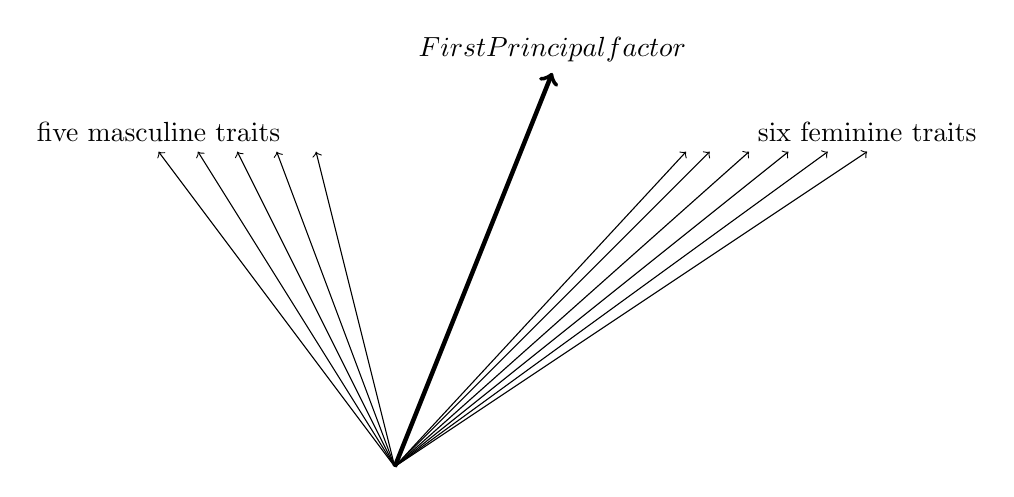
\begin{tikzpicture}
\draw[->, ultra thick, black] (0,0) -- (2,5) node[above]{$First Principal factor$};
\draw[->](0,0) -- (-3,4) node[above]{five masculine traits};
\draw[->](0,0) -- (-2.5,4);
\draw[->](0,0) -- (-2,4);
\draw[->](0,0) -- (-1.5,4);
\draw[->](0,0) -- (-1,4);
\draw[->](0,0) -- (6,4) node[above]{six feminine traits};
\draw[->](0,0) -- (5.5,4);
\draw[->](0,0) -- (5,4);
\draw[->](0,0) -- (4.5,4);
\draw[->](0,0) -- (4,4);
\draw[->](0,0) -- (3.7,4);
\end{tikzpicture} 
\caption{Finding the principal factor that explains all variation}
\label{figure:principalfactor}
\end{figure}

Once the principal component is found, the statistical software will then go ahead and try to extract a second factor, the second principal component,
which explains the remaining variation that was not explained by the first vector. This second principal component must be perpendicular to the first.
Figure ~\ref{figure:secondprincipalfactor} shows the addition of the second prinipal factor. In our case, since only two factors had an eigenvalue that
is greater than one, the software decided to stop there and concluded that the first two principal factors are enough. Since the first factor was
the one that explained as much variation as possible for all items, the result as that almost all of the items had a sufficiently large loading
on that factor (Table ~\ref{table:factormasculinefeminine}). The second principal component was then computed in order to account for the remaining
unexplained variation. Since the first factor had already accounted for much of the variation, only some of the items ended up with sufficiently
large loadings on the second principal component. 

\begin{figure}[!h]
\centering
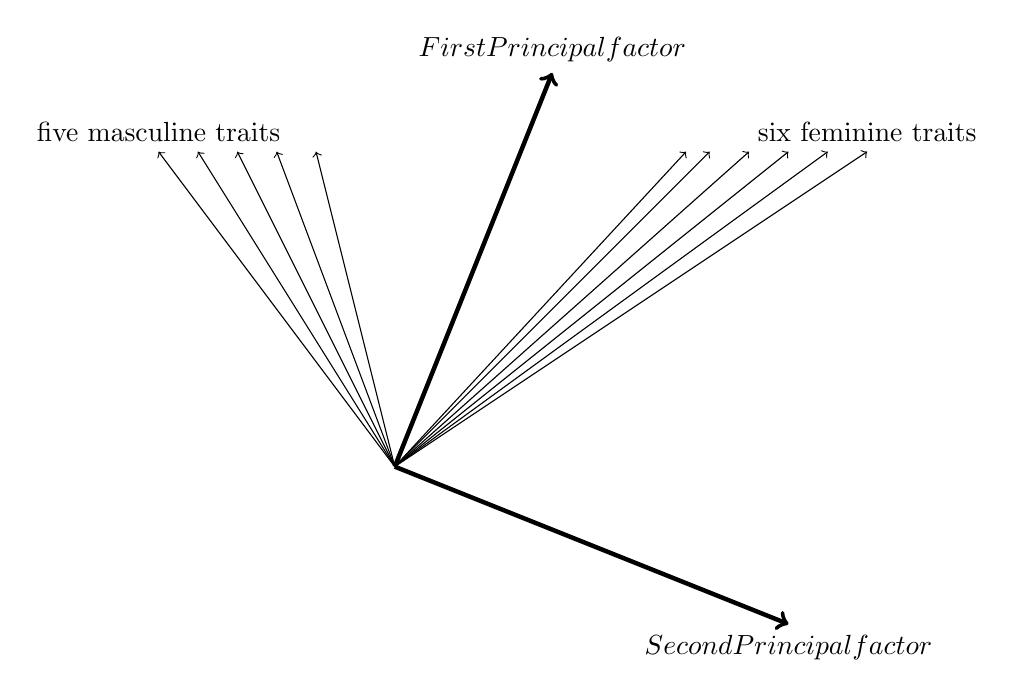
\begin{tikzpicture}
\draw[->, ultra thick, black] (0,0) -- (2,5) node[above]{$First Principal factor$};
\draw[->, ultra thick, black] (0,0) -- (5,-2) node[below]{$Second Principal factor$};
\draw[->](0,0) -- (-3,4) node[above]{five masculine traits};
\draw[->](0,0) -- (-2.5,4);
\draw[->](0,0) -- (-2,4);
\draw[->](0,0) -- (-1.5,4);
\draw[->](0,0) -- (-1,4);
\draw[->](0,0) -- (6,4) node[above]{six feminine traits};
\draw[->](0,0) -- (5.5,4);
\draw[->](0,0) -- (5,4);
\draw[->](0,0) -- (4.5,4);
\draw[->](0,0) -- (4,4);
\draw[->](0,0) -- (3.7,4);
\end{tikzpicture} 
\caption{Finding the second principal factor that explains the remaining variation}
\label{figure:secondprincipalfactor}
\end{figure}

The above visual explanation helps us understand what goes on when the software is finding the principal components. Now comes the issue of rotation.
Figure ~\ref{figure:secondprincipalfactor} shows the first and second principal components. The problem is that when the first component was extracted
the software was attemtping to explain the variation in all items at the same time. Rotation is used in order to position the principal components
in a more meanigful way. Imagine that we now rotate the first and second principal components anti-clockwise. This rotation is illustrated in 
Figure ~\ref{figure:rotate}. We now have a more accurate representation of the factors where we see that each factor represents the two different 
clusters of items. 

\begin{figure}[!h]
\centering
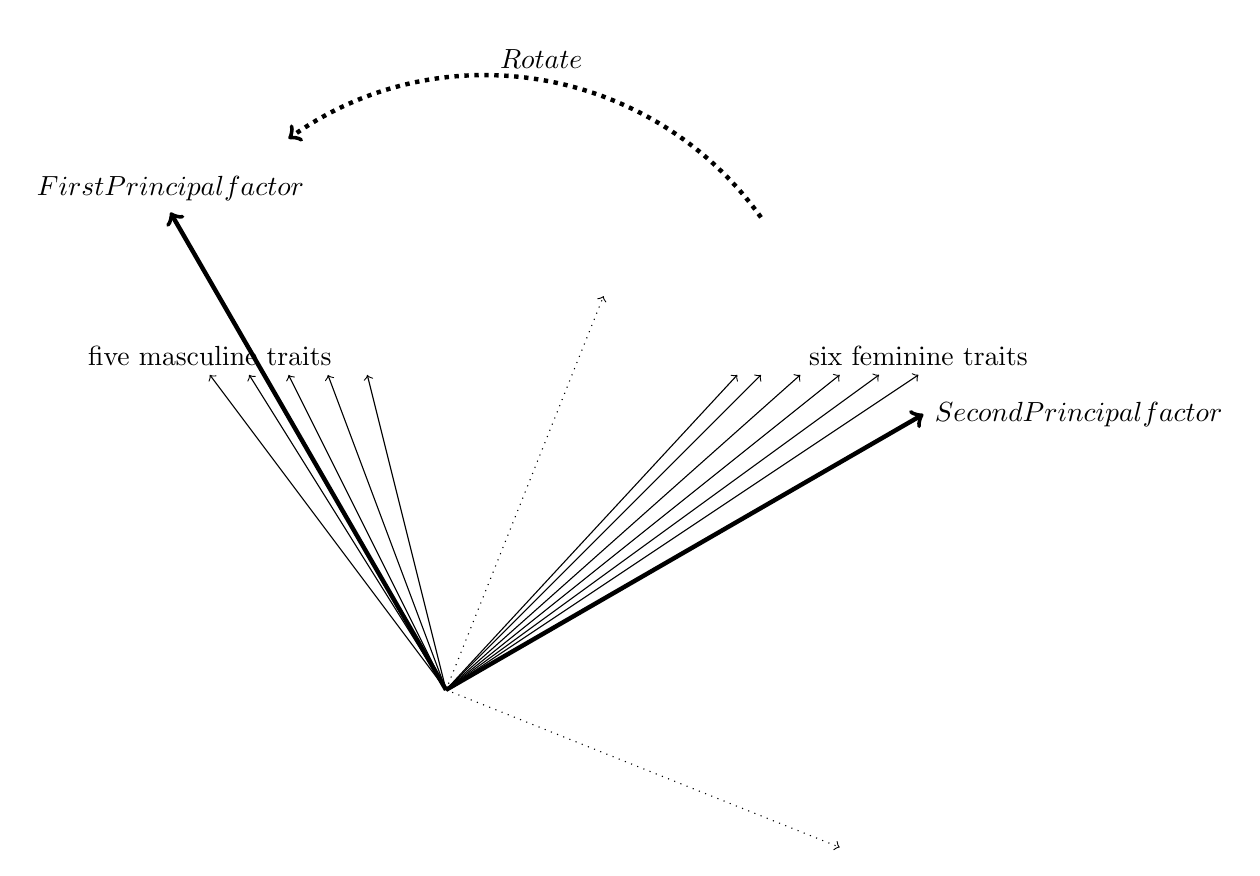
\begin{tikzpicture}
\draw[->, dotted, black] (0,0) -- (2,5);
\draw[->, dotted, black] (0,0) -- (5,-2);
\draw[->, ultra thick, black, rotate=30] (0,0) -- (0,7) node[above]{$First Principal factor$};;
\draw[->, ultra thick, black, rotate=30] (0,0) -- (7,0) node[anchor=west]{$Second Principal factor$};;
\path[->] (4,6) edge [ultra thick, dotted, black, bend right=45] node[above]{$Rotate$} (-2, 7);
\draw[->](0,0) -- (-3,4) node[above]{five masculine traits};
\draw[->](0,0) -- (-2.5,4);
\draw[->](0,0) -- (-2,4);
\draw[->](0,0) -- (-1.5,4);
\draw[->](0,0) -- (-1,4);
\draw[->](0,0) -- (6,4) node[above]{six feminine traits};
\draw[->](0,0) -- (5.5,4);
\draw[->](0,0) -- (5,4);
\draw[->](0,0) -- (4.5,4);
\draw[->](0,0) -- (4,4);
\draw[->](0,0) -- (3.7,4);
\end{tikzpicture} 
\caption{Rotating the principal components}
\label{figure:rotate}
\end{figure} 

Once we rotate the factors, we will get the loadings that are shown in Table ~\ref{table:rotatefactormasculinefeminine}. Looking at the table, we
finally see the results that we were expecting. The items assertive, competitive, dominant, makes decisions easity, and individualistic have a
loading that is greater than 0.4 on one factor (factor 2) with all corresponding loadings on the other factor (factor 1) being less than 0.4. The remainign items on the
other hand (affectionate, compassionate, gentle, understanding, sympathetic, and sensitive) have loadings that are greater than 0.4 on factor 1 while
having small loadings on factor 2. We now see that the different groups of items load on different factors. This is the result that we were
expecting.  

\begin{table}[h!t]
	\caption{Loadings of the traits after rotation.} \label{table:rotatefactormasculinefeminine}
	\centering
	\begin{tabular}{c c c}
	\hline
	{Variable} & {Factor1} & {Factor2} \\
	\hline
	assertive & 0.2033 & 0.6649\\
	competitive & 0.3153 &  0.5824\\
	dominant & 0.0160 &  0.7945\\
	individualistic & -0.0262 & 0.6405 \\
	makes decisions easily & 0.0636 & 0.6897 \\
	affectionate & 0.7109 & 0.2390 \\
	compassionate & 0.7570 & 0.1278 \\
	gentle & 0.7696 & -0.0108 \\
	understanding &  0.6409 & 0.0762 \\
	sympathetic & 0.7342 & 0.0368 \\
	sensitive & 0.6924 & 0.0546 \\
	\hline
	\end{tabular}
\end{table}

\subsection{Types of Rotation}

As discussed above, when there is more than one factor, we need to rotate the extracted factors in order to try to have each factor represent a 
cluster of items. How do we rotate the factors? Do we rotate them by ten degrees? Thirty degrees? This is a crucial question because the answer
will affect the final loadings of each item on each factor. In general, there are two types of rotation, \textbf{orthogonal} and \textbf{oblique}. 
The difference between the two types is actually simple and can be explained by looking at Figure ~\ref{figure:rotate}. In
orthogonal rotations, the factors are assumed to be independent. This means that geometrically they have to be perpendicular to each other. In
oblique rotations on the other hand, the assumption is that the factors are not independent. This means that they are not perpendicular. 

Within each type of rotation, there are several approaches. The three main orthogonal approaches are Varimax, Quartimax, and Equamax.  
As social scientists, we do not need to know the mathematical differences for each. The main thing to know is that the most commonly used 
orthogonal approach is varimax. 

The assumption that the factors are independent is actually a very strong one and in many cases it is not met. This is why some researchers
prefer oblique rotations. It happens more often than none that the factors that we are dealing with are conceptualy different but are nonetheless
correlated with each other. There are many approaches to oblique rotations such as Oblimin, Promax, and Orthoblique. The most popular methods
are Oblimin and Promax. 

So which type of rotation should we use? The answer lies in the researcher's knowledge of what is being measured. If the researcher beleives that
the factors are independent of one another, then orthogonal rotation can be used. If the researcher believes that the factors are somehow correlated
then oblique rotation can be used. In our case, we have been measuring masculinity and femininity. If you beleive tha these two constructs are
dependent (the more masculine you are then the less feminine you are) then an oblique rotation would be suitable. If, on the other, hand you 
beleive that the the two constructs are not correlated (a person can be masculine and feminine or a person can be masculine but not feminine) then
an orthogonal rotation can be used. In general, a good literature review would reveal to you what type of rotation is suitable.

To illustrate, let us continue to use the example of Masculinity and Femininity that we have been using so far. If we perform principal component
analysis on the dataset we will get the results previously displayed in Table ~\ref{table:factormasculinefeminine}. Let us know perform both an
orthogonal rotation and an oblique rotation on the factors. The results are displayed in Table ~\ref{table:rotationsboth}.

\begin{table}[h!t]
	\caption{Ortogonal and Oblique rotations.} \label{table:rotationsboth}
	\centering
	\begin{tabular}{c |c c |c c|}
	\hline
	{} & \multicolumn{2}{|c|}{Orthogonal} & \multicolumn{2}{|c|}{Oblique} \\
	\hline
	\bf Item & \bf Factor1 & \bf Factor2 & \bf \bf Factor1 & \bf Factor2 \\
	assertive & 0.2033 & 0.6649 & 0.1318 & 0.6544 \\
	competitive & 0.3153 &  0.5824 & 0.2553 & 0.5578 \\
	dominant & 0.0160 &  0.7945 & -0.0735 & 0.8075 \\
	individualistic & -0.0262 & 0.6405 & -0.0991 & 0.6554  \\
	makes decisions easily & 0.0636 & 0.6897 & -0.0133 & 0.6954 \\
	affectionate & 0.7109 & 0.2390 & 0.6971 & 0.1634 \\
	compassionate & 0.7570 & 0.1278 & 0.7566 & 0.0449 \\
	gentle & 0.7696 & -0.0108 & 0.7852 & -0.0977 \\
	understanding &  0.6409 & 0.0762 & 0.6442 & 0.0054 \\
	sympathetic & 0.7342 & 0.0368 & 0.7437 & -0.0453 \\
	sensitive & 0.6924 & 0.0546 & 0.6991 & -0.0224 \\
	\hline
	\end{tabular}
\end{table}    

Looking at Table ~\ref{table:rotationsboth}, we see that the results are almost the same. We see that the loadings of each item on each factor
are very similar in magnitude when we compare the results obtained after each type of rotation. This bascially means that the assumption that the
two factors are independent is actually valid, because when we relaxed this strict assumption by using the oblique rotation we got almost the same
results.   

\section{Recap}
The main points about factor analysis can be summarized as follows:
\begin{itemize}
	\item Factor analysis is used when we beleive that multiple items can be represented by a single factor. The two types of factor analysis are
	prinicpal component analysis and common factor analysis. The difference between the two is that principal component analysis tries to account 
	for all the variance that is observed in the items while common factor analysis tries to account only for the variance that the items share in 
	common. The more widely used method is principal component analysis.  
	\item Items have loadings on factors where each loading represents the relevance of the item to that factor. The higher the loading, the
	larger the correlation between the factor and the item. Loadings that are greater than 0.4 are considered to be substantial.
	\item We can also measure whether the items are actually measuring the same construct by calculating a reliability statistis such as
	Cronbach's alpha. A value greater than 0.7 is taken to suggest that the items are reliable.
	\item Factors with an eigenvalue greater than one are retained while factors with eigenvalues less than one are dropped. Eigenvalues are
	calculated by adding the total loadings of each item on a factor. The larger the sum, the more that a factor is correlated with the items.
	\item If the factor analysis reveals that there is more than one factor, then we need to rotate the factors. This is necessary in order to allow
	different factors to represent different clusters, especially since the first step in extracting the factors tries to find a single factor that
	accounts for the variation in all items. By rotating the factors, we are adjusting for this and allowing a more sensical interpretation of each
	factor.
	\item The two types of rotation are orthogonal and oblique. In orthogonal rotation the factors are assumed to be independent (perpendicular to
	each other) while in oblique rotation the assumption is that the factors are not independent (not perpendicular to each other). The most
	commonly used ortjogonal rotation is Varimax while the most commonly used oblique rotations are Oblimin and Promax. The choice of which rotation
	is to be used should be guided by your knowldge of the constructs being measured and by performing a suitable literature review. 
	\item Once the factors are rotated, we will have the loading of each item on each factor. This will enable us to calculate the factor score for
	each of the item. This will allow us to ask all sorts of questions, as in "Are there gender differences?" since we have a variable that records
	the gender of the respondent. If we had a variable that recorded the age of the respondent then we could have investigated whether there are
	differences in masculinity and feminity when it comes to age. 
\end{itemize}

\chapter{Factor Analysis - Case Study}
\section{The Dataset}
Let us now see how the concepts discussed in the theory part are applied when we are dealing with a dataset. In this chapter we will be using a
dataset that has been collected from questionnaires that were distributed in several schools. To understand what sort of data was being collected, 
it is important to have some information about the litterature that deals with career choices.

If you look at any university in the world, you will likely notice that female students outnumber male students in majors such as education while
male students outcumber female students in majors such as engineering. In fact, male students tend to severely outnumber female students in
what is collectively referred to as STEM fields (science, technology, engineering, and math). This led researchers to ask the natural question, "why?".
One of the most popular explanations proposed is called Social Cognitive Theory (SCT). This theory argued that females gravitate away from STEM 
fields because they beleive that they are not good at them, i.e. they have a low level of self-efficacy when it comes to these fields, at least
lower than male students. SCT argues that self-efficacy develops from four sources of information:

\begin{itemize}
	\item Mastery experience: Mastering a subject requires repeated and continuous attempts, and if girls shy away from math then they will not give
	themselves the chance to master the necessary skills. Why do girls shy away from math? Research has shown that girls have a heightened sense
	of anxiety when it comes to math.
	\item Vicarious experience: Seeing similar people successfully perform a task enhances an individual’s belief in his or her own abilities in 
	performing the task. If you take a look around you, you will notice that most engineers and mathematicians are male. Therefore, young girls do
	not see people similar to them in such positions.
	\item Social persuasion: Studies have shown that girls and boys receive different information from their surroundings with boys being encouraged
	to study math and engineering while girls ae discouraged from seeking a career in these fields in favor of careers as teachers for example.
	\item Physiological state: Studies have shown that girls have a more negative attitude towards math in general than boys. 
\end{itemize}

How can we measure these constructs? How can we assign a numerical value to "Mastery experience" for example? As you can see, this is not a 
straight-forward thing to do. In order to measure each of the four constructs, we can envision asking the respondent a series of questions where
each question will help us measure a certain aspect. This is exactly what Usher and Pajares (2009) did. In order to test the above, Usher and 
Pajares (2009) developed a questionnaire that contains 24 items where the items are intended to measure each
of the above four constructs. Table ~\ref{table:factorsurvey} shows the items used in the survey grouped by the construct which they are intended
to measure. Respondents were asked to answer each question on a scale of one to five where one indicates "strongly disagree" and 5 indicates 
"strongly agree". 

\begin{table}[!htbp]
	\caption{The 24 item questionnaire.} \label{table:factorsurvey}
	\centering
	\begin{tabular}{l|p{.95\textwidth}|}
	\hline
	{} & {How well do you agree with the following statements:} \\
	\hline
	\multirow{6}{*}{\rotatebox[origin=c]{90}{Mastery experience}} & I make excellent grades on math tests \\
	& I have always been successful with math \\
	& Even when I study very hard, I do poorly in math \\
	& I got good grades in math on my last report card \\
	& I do well on math assignments \\
	& I do well on even the most difficult math assignments \\
	\hline
	\multirow{6}{*}{\rotatebox[origin=c]{90}{Vicarious experience}} & Seeing adults do well in math pushes me to do better \\ 
	& When I see how my math teacher solves a problem, I can picture myself solving the problem in the same way \\ 
	& Seeing kids do better than me in math pushes me to do better \\ 
	& When I see how another student solves a math problem, I can see myself solving the problem in the same way \\
	& I imagine myself working through challenging math problems successfully \\
	& I compete with myself in math \\
	\hline
	\multirow{6}{*}{\rotatebox[origin=c]{90}{Social persuasion}} & My math teachers have told that I am good at learning math \\ 
	& People have told me that I have a talent for math \\ 
	& Adults in my family have told me what a good math student I am \\
	& I have been praised for my ability in math \\ 
	& Other students have told me that I’m good at learning math \\ 
	& My classmates like to work with me in math because they think I’m good at it \\ 
	\hline
	\multirow{6}{*}{\rotatebox[origin=c]{90}{Physiological state}}& Just being in math class makes feel stressed and nervous \\ 
	& Doing math work takes all of my energy \\ 
	& I start to feel stressed-out as soon as I begin my math work \\ 
	& My mind goes blank and I am unable to think clearly when doing math \\
	& I get depressed when I think about learning math \\ 
	& My whole body becomes tense when I have to do math \\
	\hline
	\end{tabular}
\end{table}

Let us take a look at the first group of items which are intended to measure the construct "Mastery experience". The first questions asks whether the
respondent gets excellent grades at math. This makes sense since it indicates that the student has mastered the subject. The second question asks
the student to indicate whether they have alwats been successful at math. Again, it makes sense that this questions measures mastery experience.
The third question is different because unlike the first two it is asking the respondent to indicate how poor they are at math. Since individuals
were asked to rate to what extent they agreed or disagreed with each statement, individuals with a high level of mastery experience will respond with
a 4 or 5 for the first two questions but will respond with a 1 or 2 for the third question. In other words, the third question is negatively
correlated with the first two. We will see later how this negative correlation manifests itself in the results. 

In addition to the 24-items, the dataset contains information about the gender and the age of the respondent. It would be interesting to see whether
these two variables are somehow correlated with the four constructs. The entire dataset contains information about 435 students.

\section{Reliability - Cronbach's Alpha}
As a first step, we would like to test whether the items are reliable or not. As you recall, this can be achieved by calculating Cronbach's alpha
and seeing whether it is greater than 0.7 or not. We do this for each group of items as shown below. 

\begin{stlog}\input{book_3.log.tex}\end{stlog}

In our dataset the questions are names math1, math2, math3,...,math24 where the first six pertain to mastery experience, the next six pertain to
vicarious experience, and next six pertain to social persuasion, and the last six pertain to physiological state. Looking at the above
output, we see that all four sets of questions have a Cronbach's alpha that is greater than 0.7. Therefore, the results so far indicate that the
items have acceptable reliability.

\section{Extracting the Factors}
Next we want to do is to investigate whether the questions do what they were intended to do. In other words, do these 24 questions
measure four different constructs? To answer this question, we need to perform factor analysis. As you recall, there are two types of factor analysis,
principal component analysis and common factor analysis. We will go ahead to perform principal component analysis for two reasons. First, it is
the most widely used option by far. Second, the researchers who developed the 24 questions themselves used principal component analysis in their
original study. If we ask te statsitical software to perform prinipal component analysis on the 24 items, we will get the output that is shown
below. 

\begin{stlog}\input{book_4.log.tex}\end{stlog}

Notice that in the first part of the output the software extracted 24 factors. As you recall, in factor analysis, the number of factors that are 
originally extracted is equal to the number of items. The table also shows the eigenvalue of each factor. We notice that only three factors have an
eigenvalue that is greater than one. This is actually unexpected, because the 24 items are intended to measure four constructs. Therefore, we would
have expected to find that four factors have an eigenvalue that is greater than one. Looking at the eigenvalue of the fourth factor, we actually see
that it is very close to one (0.98423). This is something that you will have to get used to in factor analysis, and it is that the results will
almost never be "clean". Statistical softwares are programmed to ignore factors with an eigen value less than one. This is why if you look at the
bottom table in the output you will notice that the software has calculated the loading of each item on the first three factors only. Given that the
eignevalue of the fourth factor is very close to one, and given that previous research has strongly supported the measurement tool developed by
Usher and Pajares (2009), we will tell the software to include the fourth factor.

\begin{stlog}\input{book_5.log.tex}\end{stlog}

We now see that in the bottom part of the output the software calculates the loadings on each of the first four factors. 

\section{Rotation}
Now that we have extracted the four factors, we need to rotate them in order to allow each factor to represent the diferent cluster of items.
This raises the question, how do we rotate the factors? As mentioned in the theory part, we need to decide whether we will use an orthogonal rotation
or an oblique rotation. The difference is that the orthogonal rotation assumes that the factors are independent from one another while the oblique
assumes that the factors are not independent. So which is it? If you think about it, we would expect that mastery experience and social persuasion
be correlated. If an infividual's social surrounding encourages him or her to to do something, then chances are that the individual will perform
the activities and this would increase his or her mastery of these activities. We would also expect that an individual would feel positive about
things that they are good at. Therefore, there is reason to believe that mastery experience is also correlated with physiological state. Given the
above, using an oblique rotation would make more sense. Again, there are several types of oblique rotations. Among the most popular are Oblimin, 
Promax, and Orthoblique. Usher and Pajares (2009) themselves used a Promax rotation. Therefore, it would make sense to follow their lead. 

\begin{stlog}\input{book_6.log.tex}\end{stlog}

We now have our rotated factors together with the loading of each item on each of these factors. 

Let us now take a look at the loadings in order to see whether each of the four groups of items load on one of the factors. Let us start with the 
first six items which are supposed to measure mastery experience. We see that these six items have loadings with magnitudes greater than 0.4 on the
second factor while their loadings on the other factors are less than 0.4. This is a very good result and it strongly supports the idea that the
first six items are measuring the same construct, which is different from the other three constructs. We therefore conclude that the second factor 
represents the construct mastery experience.Note however that the loading of the third item, 
math3, is negative. This is due to the fact that lower responses (1 or 2) for this item indicate a high level of mastery while larger responses (4 or
5) indicate a low level of mastery. This can be seen by looking at the question for this item which is "Even when I study very hard, I do poorly in 
math". In other words, this item is negatively correlated with the construct that we are trying to measure. In such a case, the loading will be
negative. The magnitude of the loading (the absolute value) is greater than 0.4. This means that there is a strong but opposite relationship
between this item and the construct being measured. The magnitude of the loading tells us about the strength o fthe relationship while the sign of the 
loading tells us about the direction. 

Moving on to the second set of six items (math7 to math12), we see that the first four have loadings that are greater than 0.4 on the fourth
factor while having small loadings on the other factors. The problem is that the items math11 and math12 do not load on the same factor. Instead,
math11 has its largest loading on the second factor while math12 has its largest loading on the first factor. In addition, the largest loading
of math12 is 0.3414 which is less than 0.4. This means that this item does not load sufficiently on any of the factors. We will get back to this
after we take a look at the other items. 

Mocing on to the six items that are intended to measure social persuasion (math13 to math18), we see that they all load on the first factor with 
loadings that are greater than 0.4 while their loadings on the other three factors are less than 0.4. Again, this is a good result and we therefore
conclude that the first factor represents social persuasion.

Finally, the last six items (math19 to math24) have loadings that are greater than 0.4 on the third factor. Their loadings on the other factors
are less than 0.4. Hence we conclude that the third factor represents physiological state. 

What do we conclude from the above? The results are actually pretty good. First, we extracted three items with an eigenvalue that is greater than
one, and then we managed to include a fourth because its eigenvalue was very close to one. Second, Cronbach's alpha indicates a high level of
reliability. Second, out o fthe 24 items, 22 loaded as we had expected with each grouo loading on a different factor therey indicating that the four
constructs are actually separate. What about the two items that did not load as expected? As stated above, factor analysis rarely produces clean
results. I have personally never analyzed a dataset that contains a large number of items where everything turned out perfect. Looking at the overall
picture, we see that our data provides strong support for the use of this 24-item questionnaire in measuring the four sources of information from
which mathematicla self-efficacy develops. 

\section{The Scores}
Now that we have our four factors, we can instruct the statistical software to calculate the score of each individual on all four factors. This way
we will have a four numbers per individual where these numbers are measures of the individuals mastery experience, vicarious experience, social
persuasion, and physiological state.

Let us take a look at the mean of each construct for both girls and boys.

\begin{stlog}\input{book_7.log.tex}\end{stlog}

We see that the mean for boys for the constructs mastery experience, social persuasion, and physiological state are larger than the mean for girls. This means that
on average, boys report higher levels of mastery in math, and a higher level of persuasion
from their social surroundings. With regards to physiological state, as you recall, this construct
measure how negative the attitude is towards math. If you look at the items that measure this construct (reporoduced in Table ~\ref{table:physiological} 
for ease of reference) you will notice that individuals who agree more with these items have higher levels of negative feeings towards math. This
means that higher values of this construct indicate higher levels of negative attitudes. Our results suggest that boys have a higher mean than 
girls which means that on average boys report higher levels of anxiety when it comes to math. This is unexpected since research has found that
girls have higher levels of anxiety towards math than boys. We also see that the average for girls when it comes to the construct vicarious 
experience is higher, which is again not what the literature suggests. Overall, we see that on average boys receive more positive information from
mastery experience and social persuasion while girls receive more positive information from physicological state and from vicarious experience.

\begin{table}[!ht]
	\caption{The six items that measure the construct physiological state.} \label{table:physiological}
	\centering
	\begin{tabular}{c}
	\hline
	Just being in math class makes feel stressed and nervous \\ 
	Doing math work takes all of my energy \\ 
	I start to feel stressed-out as soon as I begin my math work \\ 
	My mind goes blank and I am unable to think clearly when doing math \\
	I get depressed when I think about learning math \\ 
	My whole body becomes tense when I have to do math \\
	\hline
	\end{tabular}
\end{table}

Although looking at the mean is useful, it is not enough. We can form a more complete picture by looking at the frequency distribution of each
construct for both gender. Figure ~\ref{fig:freqpoly} shows the frequency distribution for each construct on a separate graph while comparing the
distributions for boys and girls. Looking at the distribution of the construct mastery experience, we see that at the higher end of the scale,
the percentages of boys are higher than the percentages for girls. This indicates that a larger portion of boys than girls score at the higher 
end of the scale. We also see that at the lower end o fthe scale the percentages of girls tends to be higher. If we next look at the construct 
vicarious experience, we see that percenatge of boys at the lower end tends to be higher indicating that more boys report lower levels of this
construct. If we next look at the graph for social persuasion, we again see that a larger percentage of girls score at the lower end while a larger
percentage of boys score at the upper end. Finally, if we look at the physiological state we see that, in general, larger percantages of boys score
at the higher end than girls which indicates that boys report higher levels of anxiety since, as you recall, a higher score on this construct
means that the individual reports a higher level of anxiety when it comes to math.   

\begin{stlog}\input{book_8.log.tex}\end{stlog}
\begin{figure}[h]
    \centering
    \includegraphics[width=0.9\textwidth]{book_8.pdf}
    \caption{Comparing the frequency polygons of each construct for both gender.}
    \label{fig:freqpoly}
\end{figure}

Let us now bring age into the picture. If boys are encouraged to study math and to go into engineering as they grow up, then this might mean that
for boys, the older they get, the more positive the information that they receive. Girls on the other hand as they grow older are expected to
act more lady liek and to engage in activities that are traditionally considered feminine. In this case, we would expect that as they age, girls 
receive more negative information from the four sources of information. Let us see if this is supported by our data. To do that we first produce
a scatter plot that plots the value of each construct against the age of the respondent. Figure ~\ref{fig:factorscatter} shows the scatter plot.
Unfortunately the scatter plots are not easily read. This is due to the fact that age is recorded in increments of one and many respondents
share the same age. This is resulting in the dots forming vertical lines. Fortunately, a very useful designed that is designed for these particular 
situations is called the loess curve. This curve is simply used to smooth the scatter plots. This will allow us to see whether there are any 
patterns in the data. 

Figure ~\ref{fig:factorscatter} shows the loess curves plotted on top of the scatter plots. I have made the dots from the scatter plot slightly
transparent in order to make it easier to concentrate on the lines which represent the smoothed loess curve. 

\begin{stlog}\input{book_9.log.tex}\end{stlog}
\begin{figure}[h]
    \centering
    \includegraphics[width=0.9\textwidth]{book_9.pdf}
    \caption{Comparing the frequency polygons of each construct for both gender.}
    \label{fig:factorscatter}
\end{figure}

\begin{stlog}\input{book_10.log.tex}\end{stlog}
\begin{figure}[h]
    \centering
    \includegraphics[width=0.9\textwidth]{book_10.pdf}
    \caption{The smoothed curves.}
    \label{fig:factorscatterloess}
\end{figure}

What we see from the graphs is that the older the girl, the lower the score on mastery and vicarious experience. When it comes to boys,
we do not see that there is a lot of change in the constructs as age increases. Looking at the graph of social persuasion, we clearly see that there
is an increase for boys with age while there is a decrease for girls, thereby supporting the claim that as boys grow they are encouraged to 
pursue careers in math and engineering while girls tend to receive less and less psitive information from their social surrounding. Finally
with regards to physiological state, we see that at young ages boys report higher levels of anxiety than females, but that once the age approaches
18 years the score for females increases drastically. Therefore, although the overall average of this construct is higher for boys than it is for
girls, we see that at later stages the socre of girls exceeds that of boys. Overall, the graphs show that with age, girls report lower levels of
mastery experience, vicarious experience, and social persuasion while reporting higher levels of anxiety. The only change with age for boys is with
regards to the construct social persuasion. These results clearly support the claim that with age girls are "socialised" to gravitate away from math.

This example also illustrates the importance of taking age into consideration. Despite the finding that the average for girls of vicarious
experience is higher than that of boys, as age increases the score for girls decreases. We had also previously seen how the average for boys of
physiological state was higher than that of girls thereby indicatin gthat on average boys report higher levels of math anxiety. When we took age
into consideration we saw that between te ages of 17 and 18 girls start reporting much higher levels of anxiety.

\section{Conclusion}
The results of the analysis presented in this chapter are interesting and they clearly show how factor analysis can be used to measure certain 
constructs and to compare the values of these constructs. Before analyzing the scores of the factors, we need to make sure that the items used are
actually reliable. To do that we calculated Cronbach's alpha for each of the four constructs and found that all values were greater than 0.7. Factor
analysis was then used to check whether the 24 items loaded on four different factors. The factors were rotated using oblique rotation because
theoretically each of the factors is expected to be correlated with the others. Once the factors were rotated we saw that 22 out of the 24 items
loaded as expected while two did not. As stated previously, and it is important to stress this point, factor analysis rarely produces the exact
results that are expected or even desired by the researcher. While not perfect, our factor loadings provided strong support for the use of the
24 items to measure the four distinct yet related constructs. 

Once the factors were extracted and rotated, we were able to calculate the scores of each individual on each factor using the loadings of 
each item and the response provided by each respondent to the set of questions. Having these scores opens up and whole world of analysis for us.
We were able to compare the means of each construct for both genders, compare the distribution of each construct, and finally to investigate
whether there is a relationship between the values of the constructs and age. The result was that girls see a decline in the four sources of 
information. Boys on the other hand see a noticebale increase when it comes to social persuasion. These results shed light on why few females
choose careers in STEM fields.
   
\chapter{References}

Acock, A. C. (2013). Discovering Structural Equation Modeling Using Stata. College Station, Texas: Stata Press.

Gould, S. J. (1996). The Mismeasure of Man. New York: W.W.Norton \& Company.

Pett, M. A., Lackey, N. R., \& Sullivan, J. J. (2003). Making Sense of Factor Analysis. London: SAGE.

Usher, E. L., \& Pajares, F. (2009). Sources of self-efficacy in mathematics: A validation study. Contemporary educational psychology, 34(1), 89-101.

\end{document}
